
%% Introduction

Virtual reality combines real-time computer graphics, body-tracking devices and high-resolution visual displays to create a computer-generated virtual environment. With their ability to immerse the user into a virtual mirror of the real world, virtual environments are a powerful tool in clinical application, especially in the treatment of phobias (Riva, 2003). \\
Studies have shown anxiety disorders to be the most prevalent mental disorders (Kessler et al., 2005). Many consider exposure therapy the most effective form of treatment for specific phobias (DeRubeis and Crits-Cristoph,1998). However that may be, considering the nature of certain phobias such as fear of heights, exposure therapy involves a genuine risk of injury. Performing therapy in a virtual environment therefore can be a promising alternative to the conventional in-vivo exposure.\\ 
The efficacy of virtual reality exposure therapy (VRET) has already been demonstrated in the past. A study conducted on acrophobia compared two groups of student subjects. The first group received a graded VRET. Students of the second group were added to a waiting-list as a control group. Results showed that VRET is more effective than no treatment (Rothbaum et al.,1995). VRET was also found to be as effective as exposure in-vivo in a more recent work by Emmelkamp et al. (2002).\\
In addition to this using a virtual reality system can have a number of advantages over in-vivo exposure. First and foremost being the ability to conduct therapy inside a controlled and secure environment like a therapist's office. This also implies therapy being less time consuming and provides considerable financial benefits (Cavanagh and Shapiro, 2004). The possibility of having therapy in a more private scenario also could lead to it becoming a more attractive choice for patients, that are too anxious or fear public embarrassment. 
A recent study exploring the acceptability of virtual reality exposure and in-vivo exposure in subjects suffering from specific phobias supports this hypothesis. Seventy-six percent chose virtual reality over in-vivo exposure. In addition to this the refusal rate of 3\% for virtual reality exposure was substantially lower than 27\% for in-vivo exposure (Garcia-Palacios et al., 2007). Further epidemiological studies show a lifetime prevalence of 28.5\% for vHI and 6.4\% for acrophobia alone and only 11\% of susceptible people consulting a doctor (Huppert et al., 2013; Kapfhammer et al.,2015).\\
These results suggest that virtual reality exposure could help increase the number of people who seek therapy for phobias and therefore needs to be established in everyday clinical work.\\
In recent years there has been a lot of research on virtual reality treatment for different phobias trying just that.\\
For example a controlled study by Rothbaum et al. on aerophobia (2000) as well as a open clinical trial post-traumatic stress disorder (2001) and a study on agoraphobia (Meyerbröker et al.,2011), all of which yielded positive results.
There also have been studies on ways to control the virtual reality. In a pilot study, Levy et al. (2015) explored the possibility of a remote-controlled virtual reality. After a trial session in a neutral virtual environment the patients received a total of six therapy sessions. The first three sessions were remote-controlled virtual reality exposure therapy (e-VRET) followed by three sessions in the presence of a therapist (p-VRET). E-VRET sessions were conducted without any contact to the hospital staff. The study showed that e-VRET not only is possible but produces results equal to p-VRET. %This inevitably leads us to the idea of a entirely independent VRET. 
%To our knowledge there has not yet been any research on a form of VRET, that does not depend on external control by a therapist. A system, that is able to adapt to the mental state of the patient throughout the entirety of therapy and therefore qualify for private use.  This could help expanding the reach of exposure therapy even further.\\
Assessing the mental state of a patient is essential for the success of the therapy. A task which usually falls to the hands of the therapist and in most cases relies on a verbal communication between both parties.
%To ensure the quality of our therapy system we clearly have to provide some sort of substitute for this.\\
Past studies have shown a strong psychophysiological arousal in in-vivo exposure for different specific phobias (Nesse et al.,1985; Alpers and Sell,2007). In a more recent work Diemer et al. (2015) also confirmed physiological arousal in subjects executing a virtual height challenge. The study examined phobics and healthy controls in terms of subjective and physiological fear reactions resulting in a significant increase of subjective fear, heart rate and skin conductance level. 
%We base our hypothesis on these results and claim a independent virtual reality system, that is able to react according to changes in heart rate and electrodermal activity, is possible.\\
%The present thesis is prior to a study in cooperation with the psychiatry department of the University Clinic Saarland concerning VRET on acrophobia.
%Our goal is to prove that a closed loop virtual reality system able to operate on its own by relying only on real-time physiological data is possible. 
To prove this hypothesis, we designed a virtual environment for the treatment of acrophobia that is sufficiently adaptable to various degrees of acrophobia. We will show the effectiveness of our system based on a subjective rating as well as heart rate and skin conductance measurements. Further we will deploy our virtual environment in a closed loop virtual reality system, featuring multiple control units. We will conduct a experiment simulating the effect of real-time physiology based decision making by using a remote-controlled virtual reality.\\







%%%%%%%%%%%%%%%%%%%%%%%%%%%%%%%%%%%%%%%%%%%%%%%%%%%%%%%%%%%%%%%%%%%%%%%%%%%%%%%%%%%%%%%%



%Suffering from a specific phobia such as acrophobia can be a huge interference with daily life. Those affected are often experiencing a slow progressing self-limitation fueled by their fear resulting in a declining quality of life. For people afflicted with acrophobia a therapy can therefor be life-changing.\\
%Typically a therapy is designed to help patients face their fears and practice coping strategies resulting in reducing the fear altogether. However, conducting a traditional exposure therapy can be particularly risky for the patient.
%Virtual reality guided exposure therapy offers the possibility to treat patients in a controlled environment and eliminate the risk of injury. Furthermore virtual reality assisted treatment represents a safer and cost-efficient alternative that has great potential in improving phobia treatment based on its flexibility.\\
%For example a in-vivo therapy consists of many different steps based on the initial extent of a patients fear and requires just as many individual stimulating situations. On the contrary one well designed virtual setup can easily adapt to all therapy stages and therefor be more convenient.\\

\section{Theoretical Background}

In this chapter, we will give a brief introduction to the field of anxiety disorders, especially specific phobias and the associated therapy concept, which is exposure therapy. The first part will contain fundamentals on phobias, exposure therapy and the concept of fear. Furthermore we will elaborate on the psychophysiological influences of stress and anxiety on certain parts of the human body and functions as well as methods of determination in physiological measurement. The second part will recapitulate recent approaches on virtual reality exposure therapy and analyze existing problems. 

\subsection{Acrophobia} 
%definition of fear and specific phobias,prevalence, evolutionary 	 purpose(fight or flight),connection fear to stress
%Vertigo and nausea are only two of the symptoms many people are all too familiar with when confronted with height. Acrophobia or fear of heights is one of the most common anxiety disorders and is widespread in today's society.
%According to the work of Kapfhammer et al. (2014) roughly one third of the German population will at one point in their life be afflicted by visual height intolerance (vHI). Although  considering such high numbers it comes as a surprise that only about 11\% of susceptible individuals are willing to consult a doctor(Kapfhammer et al. 2014).
%Epidemiological research showing a peak in incidence around the second decade ( Huppert et al. 2012, Agras et al. 1969) and  

 
\subsection{Stress}
%definition of stress, ways of stress perception (eustress and distress)

\subsection{Electrodermal Activity}
%%short explanation, influences(autonomic nervous system), role as method  to register physiological correlates of mental states like stress\\
%%
%%- illustration of a typical gsr signal and explanation of its components (graph, peaks etc.) \\
%%
%%- how and where is gsr usually measured? why there?\\
%

%%- exosomatic method of recording skin conductance level and skin conductance response as method of choice ( Fowles et al. 1981)

%%- secretory theory, by tarchanoff relates EDA to sweat gland activity, supported through Darrow 1927 who showed a close relation of the sweat secretion and EDA
%%-scr begins about 1 s earlier than moisture would appear on the skin surface -> gland activity not sweat on the skin itself is critical for EDA
%%- palmar sweat glands are innervated by the sympathetic chain of the autonomic nervous system -> EDA reflects sympathetic activation

%%- Another issue of central importance concerns the psychological
%%significance of EDA. From the beginning, this
%%response system has been closely linked with the psychological
%%concepts of emotion, arousal, and attention.
%%-“Every stimulus accompanied by an emotion produced
%%a deviation of the galvanometer to a degree in direct
%%proportion to the liveliness and actuality of the emotion
%%aroused” (Peterson, 1907, cited by Neumann & Blanton,
%%1970, p. 470)
%%- Woodworth and Schlosberg ,1954: They supported this indexing relationship by noting that tonic SCL is generally low during sleep and
%%high in activated states such as rage or mental work. The
%%authors also related phasic SCRs to attention, noting that
%%such responses are sensitive to stimulus novelty, intensity,
%%and significance.






Electrodermal activity (EDA) is a collective term for all electrical phenomena in the skin, which was first introduced by Johnson and Lubin (1966). This includes active and passive electrical properties, caused by skin functions and skin structure as well as the appendages of the skin.%(Thom and Boucsein, 2013). 
The skin appendages are structures formed by skin-derived cells such as hair, nails, sebaceous glands and sweat glands. EDA is one of the most commonly used response systems in psychophysiological research. This is due to its relative ease of measurement and its sensitivity to psychophysiological states and processes. The following section will provide a brief overview of EDA, ranging from physical and psychological context to recording and quantification methods.

\subsubsection{Anatomical basis} 
This section will elaborate on the anatomical aspects of the human skin and will cover all the parts and appendages, that are needed to understand the principles of EDA. The skin or cutis is the biggest organ of the human body and inherits many different functions, which are essential for survival. It primarily acts as a selective barrier, preventing the entry of foreign matter and enables the passage of materials from the bloodstream to the exterior of the body. Other than protection, it is involved in thermoregulation, cutaneous circulation and immunologic protection.  
The anatomical structure of the skin is similar in most regions of the body. Although, specialized regions of skin, such as the palms and soles may be resembling in structure, they possess modified characteristics.%(Bolognia et al., 2003)

The human skin is composed of two clearly distinguishable layers, the epidermis that serves as a protective barrier and the dermis that provides nutrition. The cutaneous structures are vertically arranged and located on top of the subcutaneous tissue. Figure \ref{layerTab} shows a representation of each of the layers and their general spatial configuration among themselves.

\begin{figure}[ht]
\centering
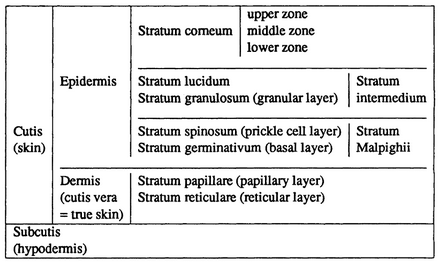
\includegraphics[width=0.8\textwidth]{images/skinLayers.png}
\caption{The Layers of the skin.The zonal layering is not so distinct in every skin region. Note that the stratum lucidum is only clearly recognizable on the palmar and plantar skin areas.\citep{boucsein2013electrodermal}}
\label{layerTab}
\end{figure}

%epidermis
The epidermis, on its own, can be divided into five different layers and lies on the surface of the skin. It consists of epithelial tissue, which is built in the lowest layer, the stratum germinativum. The main part of the produced cells are keratinocytes, which are able to store keratin and therefore become horny over time. The keratinocytes migrate to the surface of the skin, causing the epidermis to become more horny when approaching the surface. The outer layer is called the stratum corneum, originating from the fully keratinized state of its cells.
On their way to the surface the keratinocytes undergo a number of specific changes in form and areal  distribution, which in part are used to define the different epidermal layers. Also the cells become less tightly packed, compared to the deeper layers, causing the epidermis to become dryer towards the surface. A fact that greatly influences the electrical properties of the epidermis and therefore the  electrodermal activity. The stratum corneum is especially thick in the palmar and plantar regions of the body. Reaching a thickness of approximately 1 $mm$, it is almost 20 times thicker than its overall average of 50 $\mu m$.\\
%dermis
The dermis, which is also referred to as the corium, lies directly beneath the epidermis. Although it is much thicker than the epidermis it is only composed of two different dermal layers, the stratum papillare and the stratum reticulare, which are distinguishable by their density and the arrangement of their collagen fibers. The epidermal dermal junction, which is the transition area between the epidermis and dermis, resembles interlocking hands and is formed by a basal-membrane zone (Boucsein, 2013).
The dermal layer, closest to the epidermis is called the papillary stratum. Other than the capillary net of arterial and venous blood vessels, it contains receptor organs as well as melanocytes and free collagen cells. The second dermal layer, which lies on top of the subcutaneous tissue, is called the reticular stratum. It wears this name because of its texture. Formed of strong collagenous fibers, reticular stratum is highly resistant to rupture, granting the dermis is leathery impression.\\

%subcutis
The subcutis, or hypodermis, is located beneath the dermis and is composed of loose connective tissue. It serves as a connection between the skin and the connective tissue of the muscles, allowing for good horizontal mobility of the skin. The subcutis also serves as a thermal and mechanical insulation layer, due to its ability to store fat. In addition to this it, contains nerves and vessels, which supply the skin with nutrition and information, as well as the hair follicles and secretory part of the glands.   

\begin{figure}[ht]
\centering
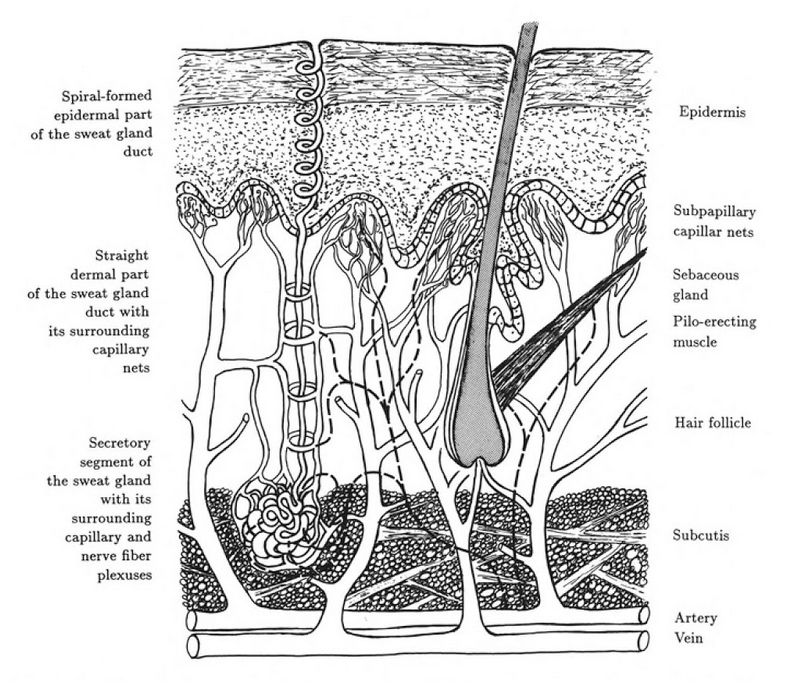
\includegraphics[width=0.7\textwidth]{images/skinDermis.png}
\caption{A artificial cross-section of the skin. It combines a sweat gland in ridged skin (left) and a hair together with a sebacous gland in polygonal skin (right).\citep{boucsein2013electrodermal}}
\label{DermisImg}
\end{figure} 

%recap link to sweat glands
The left side of figure \ref{DermisImg} shows an example for a typical profile of glabrous (hairless) skin. This specific form of skin differs in its horizontal structure. During early embryonal development specific patterns are formed by ridge formation. Ridged skin can be found on the palms of the hands and the soles of the feet. Areas, both of which, are frequently mechanically stressed and also have been found to have the highest densities of sweat glands, with an average of 233 sweat glands per $\cm^{2}$ on the hands and 620 glands per $\cm^{2}$ in adult's skin (Millington and Wilkinson 1983 in Boucsein, 2013). Sweat gland are considered to be exocrine glands, which is due to the fact that they secrete directly onto the surface of the skin. There are two types of human sweat glands, eccrine and apocrine, the majority being of the first type. The secretions of eccrine glands only contain negligible amounts of cytoplasm from the glandular cells. As there are no apocrine sweat glands located on the palmar skin, which is the most common location for EDA measurement, this section will only focus on eccrine sweat glands. The main purpose of eccrine sweat glands is to regulate the body temperature. With the exception of the palmar and plantar glands, which are thought to rather take part in grasping behavior (Edelberg, 1972, cited by Cacioppo et al., 2007). Further all eccrine sweat glands are believed to be more responsive to psychologically significant stimuli and therefore to be involved in emotional sweating. Emotional sweating is primarily observable in areas with a high density of eccrine sweat glands, such as hands and feet. Therefore, making these region particularly interesting for EDA measurement, concerning the effect of psychophysiological stimuli. Before elaborating on the connection between electrodermal activity and sweat gland activity, it is useful to consider the anatomy of the glands first.


\begin{figure}[ht]
\centering
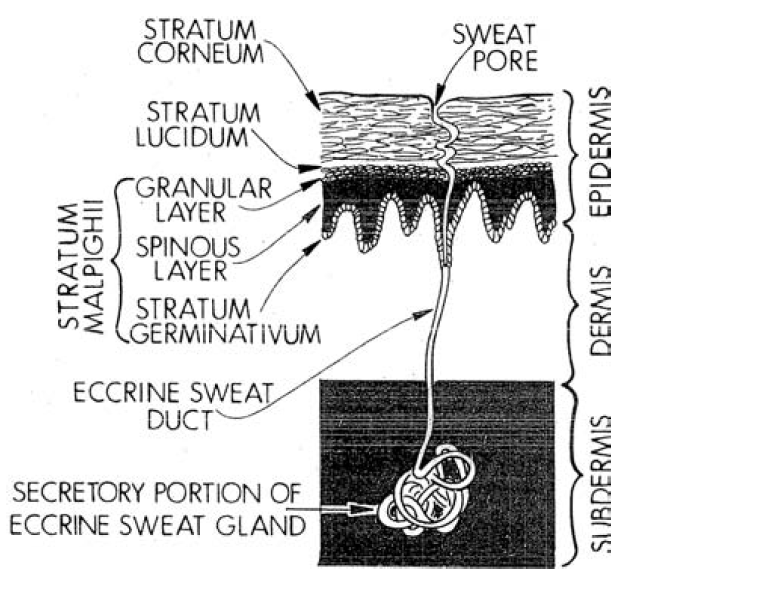
\includegraphics[width=0.7\textwidth]{images/skinAnatomy.png}
\caption{Anatomy of the eccrine sweat gland in various layers of glabrous skin.(Adapted from Hassett, 1978)\citep{HANDBOOKPP}}
\label{layerImg}
\end{figure}

Figure \ref{layerImg} shows the anatomy of an eccrine sweat gland in glabrous skin. It consists of the  secretory portion, the coiled compact body of the gland, and the sweat duct. The sweat duct, which is the excretory portion of the gland, is a long tube reaching all the way to the stratum corneum, forming a small pore on the surface of the skin. It passes through the dermis in a relatively straight line but ends up spiraling through the epidermis (Edelberg, 1972, cited by Cacioppo et al., 2007). Imagining sweat glands as a set of variable resistors wired in parallel, helps to understand their influence on electrodermal activity. As sweat rises in the ducts their electrical resistance is constantly reduced, resulting in noticeable changes in electrodermal activity. The amount of sweat and the number of glands that are currently active, and therefore the electrodermal activity depends on the degree of activation of the sympathetic division of the autonomic nervous system.

% innervation

\begin{figure}[ht]
\centering
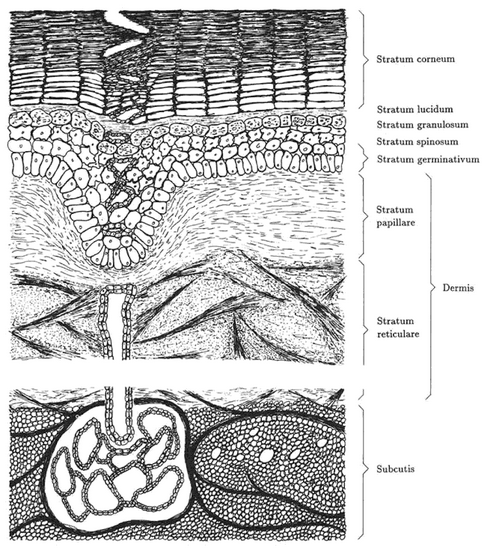
\includegraphics[width=0.7\textwidth]{images/skinGlabrous.png}
\caption{A cross-section of the layered construction of the glabrous human skin containing an eccrine sweat gland, in its glomerulus, together with its straight dermal and irregularly coiled epidermal duct. A part of the reticular layer has been omitted due to its size in relation to the rest. \citep{boucsein2013electrodermal}}
\label{layerImg}
\end{figure}

% physiology
\subsubsection{Physiological basis}
According to the previous section, focusing on the anatomical aspects, this section will outline only the physiological mechanisms required to understand electrodermal mechanisms. 
% efferent innervation of the skin
The autonomic nervous system (ANS) is a complex systems of nerves that regulates involuntary and unconscious actions. The emphasis of this section will be its thermoregulatory aspects, which also involve the skin and sweat glands. 
There are a number of efferent vegetative fibers in the human skin, including sympathetic fibers, innervating the secretory segment of the eccrine sweat glands, and vasoconstrictive efferences for the blood vessels. Originating from the brain, the efferent sympathetic nerves descend in the anterolateral part of the spinal cord in close proximity to the pyramidal tract. They are switched over in the lateral horn and leave the spinal cord through its ventral root. Alongside motoric fibers, the preganglionic sympathetic fibers travel via the white communicating ramus to the sympathetic trunk. From this point the neuronal activity will be distributed to various levels of the sympathetic trunk, causing one preganglionic fiber to reach up to 16 postganglionic neurons. The postganglionic fibers exit the sympathetic trunk through the gray communicating ramus and from there spread into the periphery, eventually reaching the skin.


% sweat gland innervation
Human sweat glands have predominantly sympathetic cholinergic innervation from sudomotor fibers originating in the sympathetic chain. The secretory part of the gland is surrounded by a dense plexus of sympathetic fibers. This allows for a wide distribution of ANS activity. The sudorisecretory fibers form a smooth bundle between the lateral pyramidal tract and the anterolateral tract. They end at the preganglionic sudorisecretory neurons and run right next to the other sympathetic fibers.  Although the sympathetic system is represented in various locations of the brain, the hypothalamus is considered to be the controlling entity of all vegetative functions. This includes sweat secretion and vasomotor activity. However, the central innervation of sweat gland activity is not limited to the hypothalamus. There are several centers, which are located in different levels of the central nervous system and partly independent of one another. The cortex, the basal ganglia, diencephalic structures such as thalamus and hypothalamus, the limbic system and brain stem areas are considered possible origins of sympathetic activity (Boucsein, 2013).

\begin{figure}[ht]
\centering
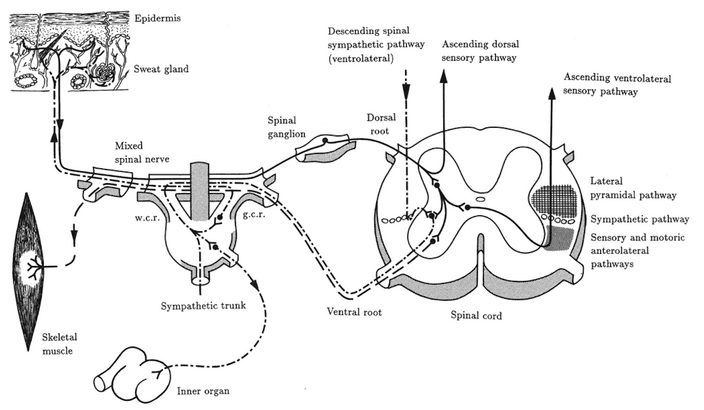
\includegraphics[width=0.7\textwidth]{images/symPathway.png}
\caption{Skin afferents and efferents at spinal cord level and connections with ascending and descending pathways. ---: motoric pathway, -.-: sympathetic efferents. \citep{boucsein2013electrodermal}}
\label{symPathImg}
\end{figure}

\subsubsection{Physiology underlying electrodermal activity}

Studies, measuring sympathetic action potentials in peripheral nerves while simultaneously recording EDA, have shown a high correlation between bursts of sympathetic nerve activity and the phasic skin conductance response (Wallin, 1981 in Cacioppo et al., 2007). Because there are many excitatory and inhibitory influences on the sympathetic system, located in various parts of the brain, there also are a variety of neural mechanisms and pathways involved into the central control of EDA.
In a review on CNS elicitation of EDA, Boucsein (2013) concludes that there are two different origins above reticular level, which were already suggested by Edelberg (1972): a limbic-hypothalamatic source, which is also thermoregulatory and emotionally influenced, and a premotor-basal ganglia source, eliciting electrodermal concomitants of the preparation of specific motor actions. In addition, Boucsein suggests a third reticular modulating system, mediating EDA changes appearing with variations of general arousal (see figure \ref{znsImg}). Further, an inhibitory EDA system has been located in the bulbar level of the reticular formation.

\begin{figure}[ht]
\centering
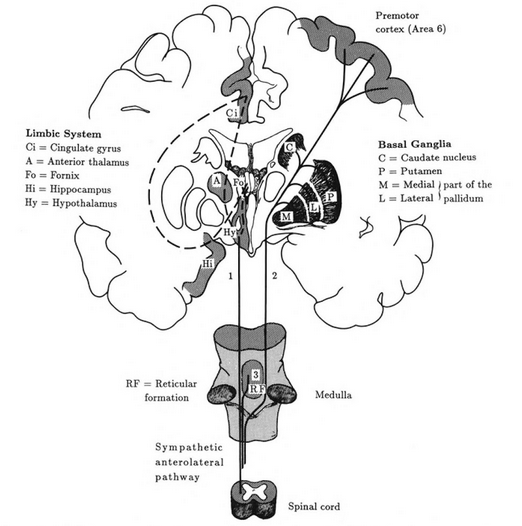
\includegraphics[width=0.8\textwidth]{images/zns.png}
\caption{Central elicitation of EDA in humans. 1: Ipsilateral influences from the limbic system via hypothalamic thermoregulatory areas; 2: Contralateral influences from premotor cortical and basal ganglia areas; 3: Reticular influences. Dashed: Connections within the limbic system.\citep{boucsein2013electrodermal}}
\label{znsImg}
\end{figure}

% properties of skin and sweat glands influencing EDA
% eda boucsein 35,36 falls sie mal wieder auftauchen
However, there are also properties of the skin, influencing the EDA, which have to be considered, especially local physiological phenomena related to sweat gland activity. Considering the vertical structure of the skin, there is a significant difference in conductivity. Both the dermis and the subcutis are tissues with strong blood supply and interstitial fluid. Therefore their elictrical conductivity is much higher than the conductivity of the epidermal layer, which forms a diffusional as well as an electrical barrier. There has been some discussion about the exact localization of an epidermal diffusional barrier, which has been reviewed in detail by Fowles (1986)(Boucsein, 2013). However, most of the findings suggest that the entire stratum corneum is forming the barrier, with the exception of its desquamating surface cells(Jarret,1980, cited by Boucsein, 2013). 
It is to mention that, under normal physiological conditions, the skin temperature is causing changes in permeability of the skin. Fowles (1986) pointed out that the permeability for water doubles with an increase in skin temperature of 7-8 $\degree C$ within the range of 25-39 $\degree C$. In spite of the diffusional barrier and without activity of the sweat glands, there is always a continuous transmission of water in the skin, directed from the dermis to the outside of the body. This causes the corneum to be always partially hydrated. However, there is a distinct relationship between the relative humidity of the air and the corneal hydration.
Thiele (1981) also showed a dependency of corneal thickness on the relative humidity of the air. As mentioned above there are differences in conductivity in the different skin layers. The barrier, formed by the outer epidermal layers, is penetrated by the sweat gland ducts, which act as diffusional and electrical shunts.
Other than these properties, concerning the resistance, living tissue has capacitative features which are related to the active its membranes. While tissue conductivity is mainly responsible for tonic EDA and, in small parts, contributes to phasic electrodermal phenomena with rather slow recovery, active membrane processes following a nerve impulse are prone to eliciting electrodermal responses with fast recovery (Boucsein, 2013).



\subsubsection{Physical recording basis}
Currently there are two basic methods of recording, the exosomatic and the endosomatic method. Whereas with the endosomatic method only changes in the potential of the skin are recorded, the exosomatic method relies on an external current to record changes in the skin resistance. This section will focus on the exosomatic method, for it being the current method of choice (Fowles et al.,1981, cited by Cacioppo et al., 2007), and describe the measurement of skin conductance level (SCL) and skin conductance response (SCR), which is the reciprocal of the skin resistance response.\\

Electrodermal activity is measured, by passing a small current through two electrodes, which are placed on the surface of the skin. The physical principal, standing behind this measurement, is Ohm's law. It states that the skin resistance (R) is equal to the voltage (V) applied between to electrodes placed on the surface, divided by the current (I) passing through the skin.
\begin{center}
\begin{equation} \label{OhmsLaw}
R = V/I \qquad ,[R] = \Omega 
\end{equation}
\end{center}

There are two concepts to current physiological recording systems. If the current is held constant then the voltage between the two electrodes can be measured. The voltage will vary directly with the skin resistance. Alternatively, if the voltage is held constant the current can be measured. The current will vary directly with the reciprocal of the skin resistance, or skin conductance. The skin conductance is expressed in units of Siemens and measures of skin conductance are usually expressed in units of micro Siemens ($\micro S$). Currently, physiological recording systems that use a constant voltage are currently the most prevalent for the direct recording of skin conductance.

\subsection{Exposure Therapy}
%what is exposure therapy?\\ 
%when is it used? \\
%how is it done?\\
%what is needed for it to be successful? \\
%how effective is it?\\
%
\section{General}
\subsection{State of the Art}
\subsection{Recent Advances in Research}
\section{Problem Analysis and Goals}
%- analyze the problem with current models of exposure therapy
%- show that my approach is different and how
%- why my approach is better and makes sense
%- goal is a safe and effective therapy option for acrophobia
%
%
